\section{Annexes}
\subsection*{Description des métriques d'évaluation d'un run et des pistes d'un run MGI dans NGL-BI}
\label{anexes1}
\subsubsection*{Liste et les description des métriques d'évaluation du run et des pistes (cf. figure \ref{NGL-screenshot_run-lane} \\page \pageref{NGL-screenshot_run-lane}) :}
\begin{itemize}
    \item[\textbf{Nb Cycles Utiles} :] Nombre de cycles des reads et des index (nombre de cyles pour le read \emph{forward}, nombre de cycles pour le premier index  \emph{forward}, nombre de cycles pour le read \emph{reverse}, nombre de cycles pour le second index)
    \item[\textbf{Nb reads (total)} :] Nombre de reads Total générer par la piste (S'il s'agit d'un run \emph{pair-end} il s'agit du nombre de cluster de reads (read \emph{forward} + read \emph{reverse}))
    \item[\textbf{\%ESR} :] \emph{Effective spot rate} ( (nombre de reads / nombre total de DNB) $\times$ 100 )
    \item[\textbf{\%q30} :] Pourcentage de bases qui ont une qualité supérieur ou égale à 30 (pour un encodage de la qualite en ASCII 33)
    \item[\textbf{\%q20} :] Pourcentage de bases qui ont une qualité supérieur ou égale à 20 (pour un encodage de la qualite en ASCII 33)
    \item[\textbf{\%q10} :] Pourcentage de bases qui ont une qualité supérieur ou égale à 10 (pour un encodage de la qualite en ASCII 33)
    \item[\textbf{\%N} :] Pourcentage de bases inconus
    \item[\textbf{Recover value} :] Rapport d'intensité entre le read \emph{forward} et \emph{reverse}
    \item[\textbf{\%Chip productivity} :] Pourcentage de productivité de la piste (nombre reads qui passent un pré-filtre MGI / nombre total de DNB)
    \item[\textbf{Nb bases} :] Nombre total de bases générés par la piste
    \item[\textbf{\%Runon1} :] Pourcentage de read \emph{forward} qui ont une incorporation de nucléotide d'avance par rapport au cycles en cours
    \item[\textbf{\%Runon2} :] Pourcentage de read \emph{reverse} qui ont une incorporation de nucléotide d'avance par rapport au cycles en cours
    \item[\textbf{\%Lag1} :] Pourcentage de read \emph{forward} qui ont une incorporation de nucléotide de retard par rapport au cycles en cours
    \item[\textbf{\%Lag2} :] Pourcentage de read \emph{reverse} qui ont une incorporation de nucléotide de retard par rapport au cycles en cours
    \item[\textbf{\%Errors} :] Pourcentage d'erreur d'incorporation de nucléotide
    \item[\textbf{\%DemultiplexingLoss} :] Pourcentage de read écartés lors du démultipléxage
\end{itemize}

% \subsection*{Description des tableaux et graphiques des rapports de séquençage des pistes d'un run}
% \label{anexes2}
% Les rapports de séquençage qui sont générés par le séquenceur contiennent trois parties, une partie résumant différentes informations à propos séquençage (\emph{Summary}), une sconde qui contient les inforamtions et graphiques à propos du \emph{Base Calling} (\emph{Basecall Information}) et la dernière partie contient les différentes statistiques et graphiques à propos des fichiers FASTQ générés (\emph{Fastq Statistics}).\\

% \subsubsection*{Description du résumé du séquençage (\emph{Summary})}

% \begin{figure}[H]
%     \centering
%     \fbox{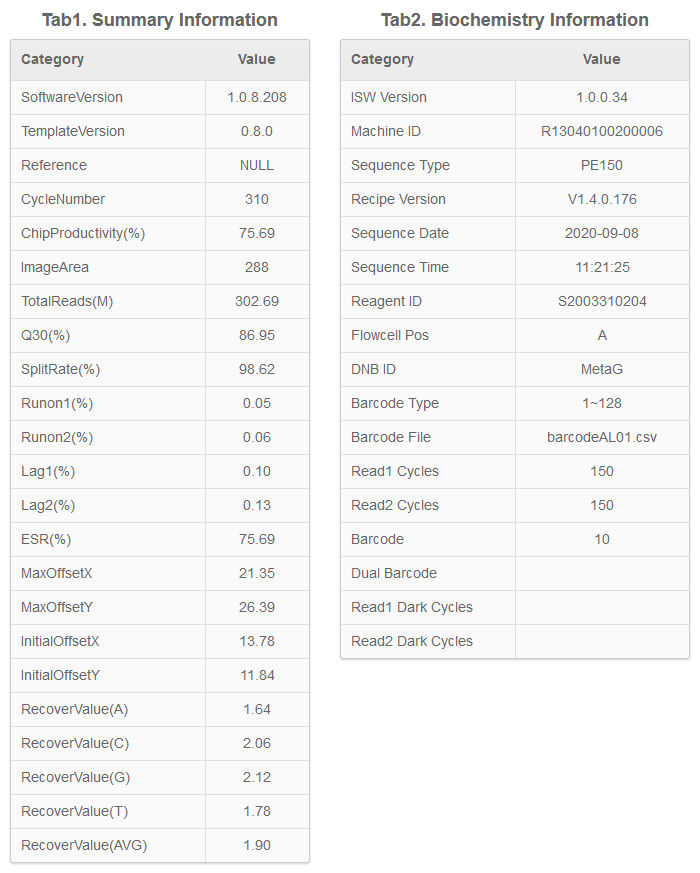
\includegraphics[width=0.6\textwidth]{img/Summary_report-html.png}}
%     \caption{\footnotesize{Capture d'écran de la page du run 200908\_MUSHU\_F300001324 de NGL en cours de génération de fichiers de séquences (onglet \og Rapport séquençage MGI\fg{})}}
%     \label{report-html-summary}
% \end{figure}

% \subsubsection*{Descriptionn des métriques et graphiques du \emph{Base calling}}

% \subsubsection*{Description des métriques et graphiques des fichiers FASTQ générés}

\newpage
\subsection*{Description des métriques d'un readset d'un run MGI dans NGL-BI}
\label{anexes3}
\subsubsection*{Liste des métriques d'évaluation des readset dans NGL\_BI (cf. figure \ref{NGL-screenshot_readset} page \pageref{NGL-screenshot_readset}) : }
\begin{itemize}
    \item[\textbf{Nb reads} :] Nombre de reads avant nettoyage des fichiers du readset
    \item[\textbf{\%déposé} :] Pourcentage d'échantillon déposé sur la piste de la flowcell
    \item[\textbf{Nb bases} :] Nombre de bases avant nettoyage des fichiers séquences du readset
    \item[\textbf{\% séquences valides/piste} :] Pourcentage de séquences de la piste appartenant à ce readset (nombre total de reads du readset / nombre total de reads de la piste)
\end{itemize}

\subsubsection*{Liste des métriques d'évaluation des readsets dans le tableau qui référence tous les readsets d'un run (cf. figure \ref{NGL-screenshot_tab-run-readset} page \pageref{NGL-screenshot_tab-run-readset}) :}
\begin{itemize}
    \item[\textbf{\%déposé} :] Pourcentage d'échantillon déposé sur la piste de la flowcell
    \item[\textbf{\% séquences valides/piste} :] Pourcentage de séquences de la piste appartenant à ce readset (nombre total de reads du readset / nombre total de reads de la piste)
    \item[\textbf{Nb Séquences valides} :] Nombre de reads du readset
    \item[\textbf{Nb Bases} :] Nombre de bases du readset
    \item[\textbf{\% >= Q30} :] Pourcentage de bases qui ont une qualité supérieur ou égale à 30 (pour un encodage de la qualité en ASCII 33)
    \item[\textbf{Score Qualité moyen} :] Moyenne de la qualité des bases du readset
\end{itemize}


\subsection*{Autres informations à propos d'un run MGI dans NGL-BI}

On retouve également les informations permettant de suivre l'avancement du workflow NGS au niveau de l'onglet \og infos workflow\fg{} (figure \ref{infos-workflow-run}).

\begin{figure}[H]
    \centering
    \fbox{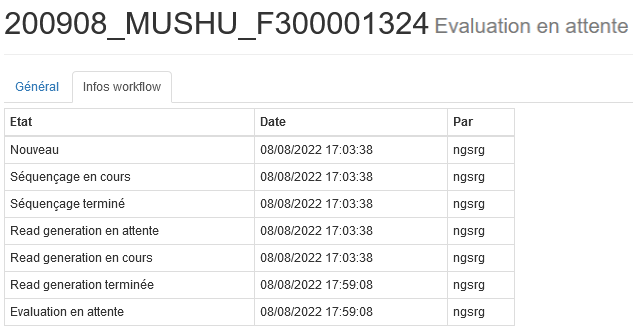
\includegraphics[width=0.6\textwidth]{img/infos_workflow_run.png}}
    \caption{\footnotesize{Capture d'écran de la page du run 200908\_MUSHU\_F300001324 de NGL en cours de génération de fichiers de séquences (onglet \og infos workflow\fg{})}}
    \label{infos-workflow-run}
\end{figure}

\subsection*{Autres informations à propos d'un readset MGI dans NGL-BI}

Il y a deux autres onglets en plus de l'onglet \og Général\fg{} et \og Avancé\fg{}. Il s'agit de l'onglet \og Infos échantillon\fg{} (figure \ref{infos-sample-readset}) et de l'onglet \og Infos workflow\fg{} (figure \ref{infos-workflow-readset}). Tout comme pour le run, l'onglet \og Infos workflow\fg{} permet de suivre l'avancement du workflow NGS pour le readset. Concernant l'onglet \og Infos échantillon\fg{}, référence toutes les informations à propos de l'échantillon du readset. On y retrouve son code, le taxon dont il fait partie et son ID, la catégorie d'échantillon (ADN, ARN \dots), la listes des barcodes utilisés et d'autres informations

\begin{figure}[H]
    \centering
    \fbox{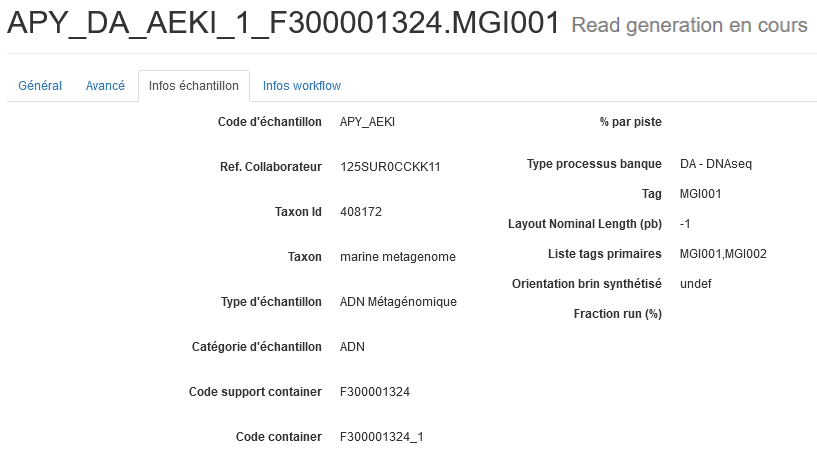
\includegraphics[width=0.6\textwidth]{img/infos_sample_readset.png}}
    \caption{\footnotesize{Capture d'écran de la page du readset APY\_DA\_AEKI\_1\_F300001324.MGI001 de NGL en cours de génération de reads (onglet \og Infos échantillon\fg{})}}
    \label{infos-sample-readset}
\end{figure}
\begin{figure}[H]
    \centering
    \fbox{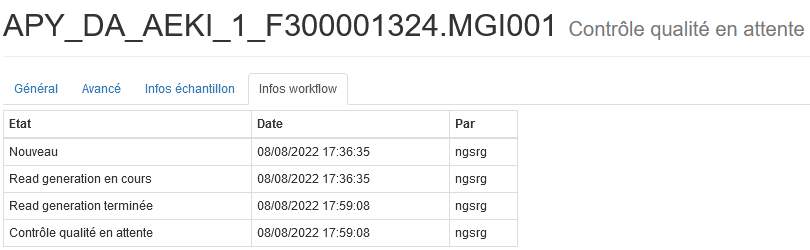
\includegraphics[width=0.6\textwidth]{img/infos_workflow_readset.png}}
    \caption{\footnotesize{Capture d'écran de la page du readset APY\_DA\_AEKI\_1\_F300001324.MGI001 de NGL en cours de génération de reads (onglet \og Infos workflow\fg{})}}
    \label{infos-workflow-readset}
\end{figure}